\documentclass[answers]{exam}

\usepackage{amsmath}
\usepackage{amssymb}
\usepackage[spanish]{babel}
\usepackage{drawstack}
\usepackage{enumerate}
\usepackage[T1]{fontenc}
\usepackage{lmodern}
\usepackage{listings}
\usepackage{graphicx}
\usepackage{semantic}
\usepackage{stmaryrd}
\usepackage[cache=false,outputdir=./build]{minted}
\usepackage{xcolor} % to access the named colour LightGray
\definecolor{LightGray}{gray}{0.9}

% paquetes para escribir algoritmos y pseudocódigo
\usepackage{algpseudocode}
\usepackage{algorithm} 
\usepackage{algpseudocode} 
\renewcommand{\algorithmicrequire}{\textbf{Input:}} % Use Input in the format of Algorithm 
\renewcommand{\algorithmicensure}{\textbf{Output:}} % Use Output in the format of Algorithm
% paquetes para escribir algoritmos y pseudocódigo

\decimalpoint{}

\newcommand{\materia}{Programación Funcional}
\newcommand{\tarea}{Tarea 1}

\firstpageheadrule{}
\firstpageheader{
  Ramírez López Alvaro\\
  Numero de cuenta: 316276355
}{
  \materia{} \\
  \tarea{}
}{
  Fecha de entrega: \\
  24 de enero de 2023
}

\extrawidth{1.54cm}
\extraheadheight[5mm]{-5mm}
\renewcommand{\familydefault}{\sfdefault}

\renewcommand{\solutiontitle}{\noindent\textbf{Solución:}\par\noindent}
\runningheadrule{}
\runningheader{\materia{}}{\tarea{}}{\today}
\footer{}{Página \thepage\ de \numpages}{}

\lstset{basicstyle=\ttfamily,tabsize=3}
\definecolor{bg}{rgb}{0.95,0.95,0.95}

\begin{document}

\begin{questions}

\question{Transforma las siguientes expresiones aritméticas en expresiones de Racket y pruébalas en el área de interacciones. 
Anota el resultado de evaluar cada expresión.
\begin{itemize}
  \item $(4 * 7) - (13 + 5)$
  \item $(3 * (4 + (-5 - 3)))$
  \item $(2.5 \div (5 * (1 \div 10)))$
  \item $5 * ((537 * (98.3 \div (375 - (2.5 * 153)))) + 255)$
\end{itemize}
}

\begin{solution}
  %% insertar imagen
  \begin{center}
    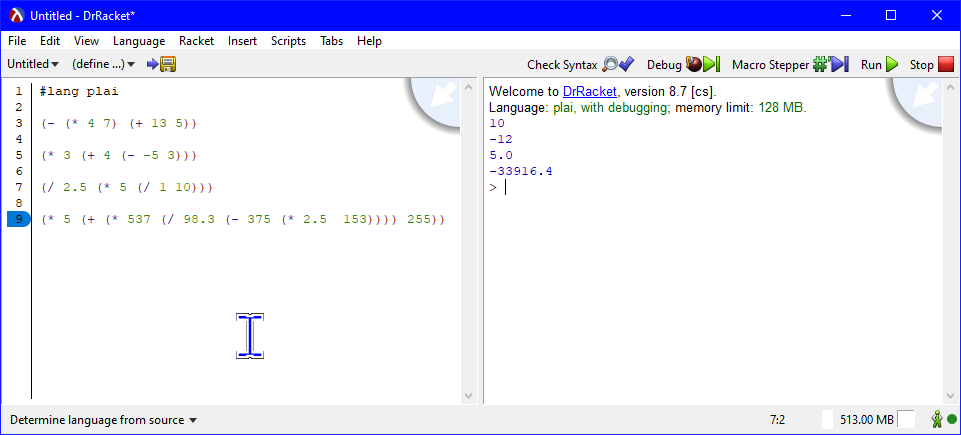
\includegraphics[scale=.65]{images/tarea1-1.png}
  \end{center}
\end{solution}

\question{Transforma las siguientes fórmulas en expresiones de Racket y pruébalas en el área de interacciones.
\begin{itemize}
  \item Ecuación general de segundo grado:
  \begin{center}
    $x_1 = \frac{-b + \sqrt{b^2 - 4ac}}{2a}$ y $x_2 = \frac{-b - \sqrt{b^2 - 4ac}}{2a}$
  \end{center}
  con $a = 3$, $b = 6$ y $c = 2$.
  \item Distancia entre dos puntos:
  \begin{center}
    $d = \sqrt{(x_2 - x_1)^2 + (y_2 - y_1)^2}$
  \end{center}
  con $x_1=5$, $x_2=-4$, $y_1=-3$ y $y_2=6$.
  \item Teorema de Pitágoras:
  \begin{center}
    $c=\sqrt{a^2+b^2}$
  \end{center}
  con $a=3.7$ y $b=5.4$.
  \item Evaluación de polinomios:
  \begin{center}
    $y=2x^3-4x^2+8x-2$
  \end{center}
  con $x=6$.
\end{itemize}
}

\begin{solution}
  %% insertar imagen
  \begin{center}
    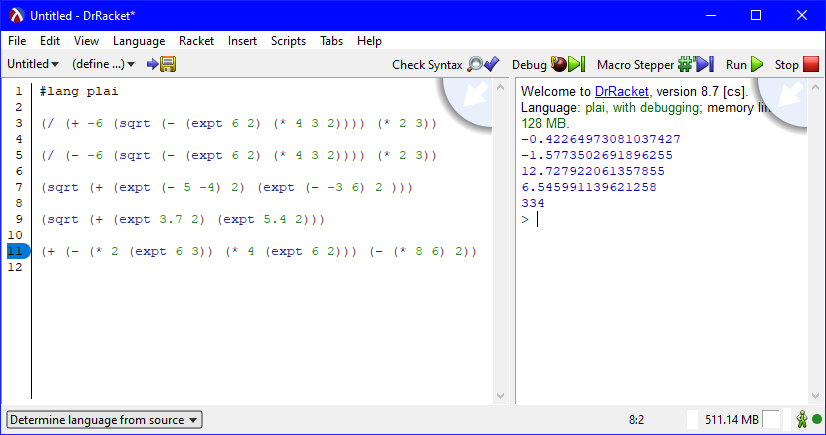
\includegraphics[scale=.65]{images/tarea1-2.png}
  \end{center}
\end{solution}

\end{questions}

\end{document}